\documentclass{beamer}

%gets rid of bottom navigation bars
\setbeamertemplate{footline}[page number]{}

%gets rid of navigation symbols
\setbeamertemplate{navigation symbols}{}

\title{Computational analysis of single-cell RNA-seq data: 
challenges, solutions and opportunities}

\author{Aaron Lun \\[0.1in]
\footnotesize{CRUK Cambridge Institute}
}

\date{
\footnotesize{Single-cell Analysis Workshop, TAU}\\[0.1in]
22 May 2018
}

\begin{document}
\maketitle

\begin{frame}{What is single-cell RNA sequencing (scRNA-seq)?}
\begin{center}
    \includegraphics[width=\textwidth]{pics/scRNAseq.pdf}
\end{center}
... using microfluidics, plate-based or droplet-based protocols
\end{frame}

\begin{frame}{Why should we use scRNA-seq?}
    \vspace{0.1in}
    Characterize heterogeneity across a cell population using transcriptome-wide expression profiles (vs. bulk, FACS) \\[0.5em]
\begin{itemize}
    \setlength\itemsep{0.5em}
    \item identify cell ``trajectories'', e.g., in differentiation
    \item define subpopulations at single-cell resolution
    \item study noise in transcriptional regulation
\end{itemize}
\pause
\begin{center}
    \begin{tabular}{c c}
        \includegraphics[width=0.39\textwidth,trim=0mm 65mm 110mm 8mm,clip]{pics/oligodendrocytes_GCB.jpg} &
        \includegraphics[width=0.49\textwidth,trim=5mm 120mm 90mm 45mm,clip]{pics/pancreas_AVO.jpg} \\
        {\tiny \textit{Science} (2016), 352:1326-1329} &
        {\tiny \textit{Cell Systems} (2016), 3:385-394.e3} \\
\end{tabular}
\end{center}
\end{frame}

\begin{frame}{What are the challenges in scRNA-seq data analysis?}
    \begin{alertblock}{What is the missing step?}
    scRNA-seq data $\to$ \uncover<2>{\textbf{computational analysis}} $\to$ interesting biology \\[0.1in]
\end{alertblock}
    \pause
    Generating a cDNA library from a single cell is \textit{hard}:\\[0.1em]
    \begin{itemize}
        \setlength\itemsep{0.5em}
        \item high dropout rates, i.e., molecule is present but not captured
        \item variable capture rates across cells
        \item low quality cells where mRNA is not captured or lost
        \item duplicated reads from PCR amplification 
    \end{itemize}
    \vspace{0.1in}
    What is genuine biology? What is technical noise? 
\end{frame}

\begin{frame}{What does scRNA-seq data look like?}
In its rawest form\footnote{Excluding BCL files.}, FASTQ files after Illumina sequencing.
\begin{enumerate}
\item Align to reference genome (e.g., STAR)
\item Count number of reads per gene (e.g., HTSeq)
\end{enumerate}
Output is a count matrix with genes as rows and cells as columns. 

\begin{exampleblock}{Exceptions and alternatives}
\begin{itemize}
    \item pseudo-aligners, e.g., Salmon, Kallisto
    \item UMI handling, e.g., with \texttt{UMI-tools}
    \item droplet data, e.g., \texttt{CellRanger}
\end{itemize}
\end{exampleblock}
\end{frame}

\begin{frame}{What does scRNA-seq data look like?}
A typical scRNA-seq count matrix:
\begin{center}
    \includegraphics[width=\textwidth]{pics/scData.pdf} \\
    \vspace{-.1in}
    {\tiny Data from \textit{Science} (2015), 347:1138-42}
\end{center}
\begin{itemize}
    \item lots of zeros due to dropout events (\textbf{or no expression!})
    \item variable total counts across cells - cell-specific biases
    \item variable counts per gene - part biological, part technical
\end{itemize}
\end{frame}

\begin{frame}{Performing a basic analysis of scRNA-seq data}
    Starting from a count matrix:\\[0.1em]
    \begin{enumerate}
        \setlength\itemsep{0.5em}
        \item Quality control on the cells
        \item Normalization of cell-specific biases
        \item Modelling technical noise 
        \item Dimensionality reduction and clustering
    \end{enumerate}
    ... followed by higher-level analyses and interpretation.
\end{frame}

\begin{frame}{Quality control on the cells}
    Low-quality cells generated by:
    \begin{itemize}
        \item insufficient sequencing
        \item failed reverse transcription
        \item damaged cells during dissociation
    \end{itemize}
    \vspace{0.1in}
    We use the following metrics to identify and remove them:
    \begin{itemize}
        \item total number of reads for each cell \textit{(low)}
        \item total number of expressed features for each cell \textit{(low)}
        \item percentage of reads mapped to spike-in transcripts \textit{(high)}
        \item percentage of reads mapped to mitochondrial genes \textit{(high)}
    \end{itemize}
\end{frame}
   
\begin{frame}{Distributions of total counts, total features}
    Various batches of human ESCs:
    \begin{center}
        \includegraphics[width=\textwidth]{pics/libSize_WR.png}
    \end{center}
    {\tiny Data from Ferdinand von Meyenn and Wolf Reik at the Babraham Institute}
\end{frame}
    
\begin{frame}{Distributions of spike-in, mitochondrial proportions}
    Various batches of human ESCs:
    \begin{center}
        \includegraphics[width=\textwidth]{pics/mitoAndSpikes_WR.png}
    \end{center}
    {\tiny Data from Ferdinand von Meyenn and Wolf Reik at the Babraham Institute}
\end{frame}

\begin{frame}{What is ``low-quality''?}
    \begin{exampleblock}{Approach 1}
        Define fixed thresholds, e.g., at least 100,000 counts per cell
        \begin{itemize}
            \item simple, easy to interpret
            \item hard to generalize across data sets 
        \end{itemize}
    \end{exampleblock}
    \pause
    \begin{exampleblock}{Approach 2}
        Detect outliers in the QC metric distribution:\\
        $\quad\hookrightarrow$ remove small outliers for total counts, features \\
        $\quad\hookrightarrow$ remove large outliers for \% of spike-in/mitochondrial reads
        \begin{itemize}
            \item adapts to mean/variance of QC metrics across population
            \item assumes most cells are high-quality, homogeneous metrics
        \end{itemize}
    \end{exampleblock}
    \pause
    \begin{alertblock}{Approach 3}
        Define low-quality cells as outliers on gene expression
        \begin{itemize}
            \item Risky, may remove cells in rare subpopulations
        \end{itemize}
    \end{alertblock}
\end{frame}

\begin{frame}{Assigning the cell cycle phase (cyclone)}
\begin{center}
    \includegraphics[width=\textwidth]{pics/phase_assign.pdf} \\
    {\tiny See \emph{Methods} (2015), 85:54-61}
\end{center}
\end{frame}

\begin{frame}{Example of a phase score plot}
    Each point is a T-helper 2 cell: {\tiny (Data from \emph{Nat. Biotechnol.} (2015), 33:155-160)}
    \begin{center}
        \includegraphics[width=0.7\textwidth,trim=0mm 7mm 0mm 25mm,clip]{pics/phase_th2_OS.png}
    \end{center}
    Scores are computed from number of pairs supporting that phase.
\end{frame}

\begin{frame}{Normalizing out cell-specific biases}
Differences in library size, capture efficiency between cells
\begin{itemize}
    \item scaling normalization to remove biases \textit{between} cells
    \item compute a ``size factor'' to divide the counts for each cell 
\end{itemize}
\vspace{0.1in}
\textbf{To demonstrate:} consider counts for a few genes in a few cells
\begin{itemize}
\item assume X, Y, Z... are \textit{not} DE between cells
\item systematic fold-differences are technical in origin
\end{itemize}

\begin{center}
\begin{tabular}{l p{0.2in} p{0.2in} p{0.2in} p{0.2in}}
\hline
& \textbf{Cell} \\
        \cline{2-5}
& \textbf{A} & \textbf{B} & \textbf{C} & \textbf{D} \\
\hline
Gene X & 10 & \alt<1>{20}{\textcolor{red}{10}} & \alt<1>{30}{\textcolor{red}{10}} & \alt<1>{40}{\textcolor{red}{10}} \\
Gene Y & 15 & \alt<1>{30}{\textcolor{red}{15}} & \alt<1>{45}{\textcolor{red}{15}} & \alt<1>{60}{\textcolor{red}{15}} \\
Gene Z & 20 & \alt<1>{40}{\textcolor{red}{20}} & \alt<1>{60}{\textcolor{red}{20}} & \alt<1>{80}{\textcolor{red}{20}} \\
& ... & ... & ... & ... \\ 
\hline
\textbf{Size factor} & 1 & 2 & 3 & 4 \\
\hline
\end{tabular}
\end{center}
\end{frame}

\begin{frame}{Composition biases due to differential expression}
\begin{center}
\includegraphics[width=\textwidth]{../introduction/pics/composition_bias.pdf}
\end{center}
\begin{itemize}
\item Normalization by library size provides no protection
\item Requires methods robust to DE, e.g., TMM, DESeq
\item ... but such methods are not robust to zeroes!
\end{itemize}
\end{frame}

%\begin{frame}{Existing methods for calculating size factors}
%\begin{itemize}
%\item \textbf{DESeq:} compare each cell to an average pseudo-cell 
%\item \textbf{TMM:} compare each cell to an arbitrary reference cell
%\item \textbf{Library size:} total sum of counts per cell as size factor 
%\end{itemize}
%
%\vspace{0.05in}
%\textbf{But...} TMM, DESeq normalization don't handle zeroes well \\
%Library size normalization doesn't deal with composition bias \\[0.1in]
%
%Simulations with DE between \textcolor{blue}{pop}\textcolor{orange}{ula}tions, lots of zeroes:
%\begin{center}
%    \includegraphics[width=0.32\textwidth]{pics/size_1_AL.pdf}
%    \includegraphics[width=0.32\textwidth]{pics/TMM_1_AL.pdf}
%    \includegraphics[width=0.32\textwidth]{pics/lib_4_AL.pdf} \\
%    {\tiny \emph{Genome Biol.} (2016), 17:75}
%\end{center}
%\end{frame}

\begin{frame}{Deconvolution: sharing information across cells}
    \begin{center}
        \includegraphics[width=\textwidth]{pics/deconvolution_AL.pdf} \\
    {\tiny \emph{Genome Biol.} (2016), 17:75}
    \end{center}
    \vspace{-0.1in}
    \begin{itemize}
        \item Pooling cells to increase counts, avoid problems with zeros.
        \item Size factor per pool estimated robustly, to protect against DE.
        \item Solve linear system to obtain a size factor \textbf{per cell}.
    \end{itemize}
\end{frame}

%\begin{frame}{Applying the deconvolution method}
%    Works well on simulated data (left):
%    \begin{center}    
%    \includegraphics[width=0.49\textwidth,trim=0mm 0mm 0mm 20mm,clip]{pics/sumClust_4_AL.pdf} 
%    \includegraphics[width=0.49\textwidth,trim=55mm 55mm 60mm 0mm,clip]{pics/Figure5_AL.pdf}
%    \end{center}
%    Makes a difference in real data (right) compared to other methods. \\[0.1in]
%    % Not totally academic; some effect from normalizing in a manner that properly handles the abundance of zeros.
%\end{frame}

\begin{frame}{Normalizing spike-ins separately}
Normalization on gene counts corrects for RNA content
\begin{itemize}
    \item counts for spike-in transcripts not affected by RNA content
    \item using gene-based size factors will ``over-normalize''
\end{itemize}
\begin{center}
    \begin{minipage}{0.49\textwidth}
        \begin{tabular}{|l|c c|}
            \hline
            \textbf{Before}
                   & Cell A & Cell B \\
            \hline
            Gene X & 10 & 20 \\
            Gene Y & 20 & 40 \\
            Gene Z & 30 & 60 \\
            Spike 1 & 5 & 5  \\
            \hline
        \end{tabular}
        \end{minipage}
    \begin{minipage}{0.49\textwidth}
        \begin{tabular}{|l|c c|}
            \hline
            \textbf{After}
                   & Cell A & Cell B \\
            \hline
            Gene X & 20 & 20 \\
            Gene Y & 40 & 40 \\
            Gene Z & 60 & 60 \\
            Spike 1 & \textcolor{red}{10} & 5  \\
            \hline
        \end{tabular}
        \end{minipage}
    \end{center}
Define sum of spike-in counts as ``spike-in size factor'':
\begin{itemize}
    \item normalize spike-ins by dividing with spike-in size factor
    \item normalize genes by dividing with gene-based size factor
\end{itemize}
\pause
\textcolor{red}{Do not use the gene-based size factors on the spike-in counts}
\end{frame}

\begin{frame}{Spike-in versus gene-based normalization}
    \vspace{0.1in}
\textbf{Alternatively:} normalize genes with spike-in size factors
\begin{itemize}
    \item when you can't assume most genes are not DE
    \item when changes in total RNA content are interesting
\end{itemize}
\begin{center}
    \includegraphics[width=0.6\textwidth,trim=0mm 8mm 0mm 22mm,clip]{pics/spikes_MEF_SL.png}\\
    {\tiny Data from \emph{Genome Res.} (2011), 21:1160-1167}
\end{center}
\end{frame}

\begin{frame}{Computing normalized log-expression values}
    For gene $g$ in cell $i$, divide count $y_{ig}$ by size factor $s_i$ to get:
    \[
        \log_2\left(\frac{y_{ig}}{s_{i}} + 1\right)
    \]
    
\begin{itemize}
    \item differences between log-values represent log-fold changes
    \item more relevant than absolute differences in counts
\end{itemize}
\begin{center}
\begin{tabular}{l l l}
\hline
& Cell A & Cell B \\
\hline
Gene X & 1000 & 1100 \\
Gene Y & 0 & 20 \\
\hline
\end{tabular}
\end{center}
Related to the concept of ``variance stabilization''
\end{frame}

\begin{frame}{Modelling technical and biological variance}
    \textbf{How much of cell-to-cell variability is technical vs biological?} \\
$\quad\hookrightarrow$ how do we quantify variance in the first place?

\begin{block}{Squared coefficient of variation (CV$^2$)}
    Divide variance of (normalized) counts by the squared mean:
    \[
        \frac{\mbox{var}(z_{ig})}{\bar{z}^2_g} \quad\mbox{where}\quad z_{ig} = \frac{y_{ig}}{s_i}
    \]
\end{block}

\begin{block}{Variance of log-expression}
    Compute variance of normalized log-expression values:
    \[
        \mbox{var}[\log_2(y_{ig}/s_i + 1)]
    \]
\end{block}

CV$^2$, logging try to eliminate the mean-variance trend...
\end{frame}

\begin{frame}{Fitting a trend to the technical variance}
    \vspace{-0.2in}
\begin{center}
    \begin{tabular}{c@{}c}
    \includegraphics[width=0.49\textwidth,trim=0mm 0mm 0mm 25mm,clip]{pics/hvg_hsc_BG.png} &
    \includegraphics[width=0.49\textwidth]{pics/brennecke_HVG.jpg} \\
    {\tiny Data from \emph{Cell Stem Cell} (2015), 16:712-724} &
    {\tiny \emph{Nat. Methods} (2013), 10:1093-1095}
\end{tabular}
\end{center}
Fit a trend to the variance of the spike-ins:
\begin{itemize}
    \item quantify variance due to technical noise only.
    \item biological variance = residual from the trend for each gene
\end{itemize}
Identify interesting genes for downstream steps = feature selection.
\end{frame}

%\begin{frame}{Detecting highly variable genes}
%\textbf{Identify most interesting genes for downstream analysis.}\\[0.1in]
%
%\textit{H$_0$: biological component of variance/CV$^2$ = 0}
%\begin{enumerate}
%    \item compute one-sided $p$-value for each gene
%    \item correct for multiple testing 
%    \item reject at a given false discovery rate to define HVGs
%\end{enumerate}
%
%\begin{exampleblock}{Which method to use?}
%    \begin{itemize}
%        \item CV$^2$ better at detecting upregulation in rare populations
%        \item Variance of logs more robust to outlier expression
%    \end{itemize}
%\end{exampleblock}
%\pause
%\begin{alertblock}{No spike-ins, what to do?}
%    Fit trend directly to variances of genes:
%    \begin{itemize}
%        \item overestimates technical noise
%        \item identify ``relatively'' highly variable genes
%    \end{itemize}
%\end{alertblock}
%\end{frame}

\begin{frame}{Dimensionality reduction with PCA}
PCA = principal components analysis
\begin{itemize}
    \item identifies axes of maximal variance in high-dimensional data
    \item each principal component (PC) explains less variance 
\end{itemize}
\begin{center}
\includegraphics[width=\textwidth,trim=0mm 5mm 0mm 40mm,clip]{pics/pca_explanation.pdf}
\end{center}
\textbf{Use the first few (5-100) PCs as a ``summary'' of the data}
\begin{itemize}
\item Speed up downstream analyses by reducing dimensionality
\item Focus on biology, remove random noise in later PCs
\end{itemize}
\end{frame}

%\begin{frame}{Selecting the number of PCs to retain}
%Use our model of technical noise to discard later components:
%\begin{center}
%\includegraphics[width=\textwidth]{pics/denoise_PCs.pdf}
%\end{center}
%Retain PCs for clustering, pseudo-time reconstruction, $t$-SNE...
%\end{frame}

\begin{frame}{Visualization with PCA}
The first 2-3 PCs can be directly used for visualization:
\begin{center}
    \includegraphics[width=0.9\textwidth]{pics/pca_brain_SL.png} \\
    {\tiny Data from \textit{Science} (2015), 347:1138-42}
\end{center}
Simple and efficient, but limited resolution of complex structure.
% Internal differences within blobs not visible, dominated by differences between blobs.
\end{frame}

\begin{frame}{Visualization with $t$-SNE}
Finds a low-dimensional representation of high-dimensional data 
\begin{itemize}
    \item preserve distances to neighbouring cells
    \item non-linear: not limited to straight axes
\end{itemize}
\begin{center}
    \includegraphics[width=0.9\textwidth]{pics/tsne_brain_SL.png} \\
    {\tiny Data from \textit{Science} (2015), 347:1138-42}
\end{center}
Powerful, but need to fiddle with random seed and perplexity
\end{frame}

\begin{frame}{Dimensionality reduction: diffusion maps}
Uses a diffusion process to model a continuum of expression
\begin{itemize}
    \item useful for trajectories (e.g., differentiation)
\end{itemize}
\begin{center}
    \includegraphics[width=0.5\textwidth]{pics/diffusion_th2_OS.png} 
    {\tiny (Data from \emph{Nat. Biotechnol.} (2015), 33:155-160)}
\end{center}
... and a lot more, e.g., SOMs, force directed graphs.
\end{frame}

\begin{frame}{A few words on clustering}
    \textbf{Aim:} To group cells with similar expression profiles \\
    $\quad\hookrightarrow$ identify and characterize new subpopulations\\[0.15in]

   Lots of algorithms:
\begin{itemize}
    \item hierarchical flavours
    \item $k$-means
    \item community detection (graph-based)
\end{itemize}
\vspace{0.1in}
Lots of distance metrics:
\begin{itemize}
    \item Euclidean
    \item cosine (i.e., Pearson's correlation, Spearman's rho)
\end{itemize}
\vspace{0.1in}
Most methods work well, provided you:
\begin{itemize}
    \item filter to only use features of interest
    \item assess cluster separatedness (silhouette width, gap statistic)
    \item experimentally validate putative clusters.
\end{itemize}
\end{frame}

\begin{frame}{Wrapping up}
    Starting from a count matrix:\\[0.1em]
    \begin{enumerate}
        \setlength\itemsep{0.5em}
        \item Quality control on cells 
        \item Normalization of cell-specific biases
        \item Modelling technical noise
        \item Dimensionality reduction and clustering
    \end{enumerate}
    ... followed by higher-level analyses and interpretation. \\[0.2in]
    \begin{center}
    \textbf{Try it yourself!}
\end{center}
\begin{block}{What's on the horizon?}
    \begin{itemize}
        \item Dealing with batch effects (see \texttt{?mnnCorrect})
        \item Handling huge data sets, e.g., 10X 1.3M neurons
        \item Integrative analysis of multi-condition data sets
    \end{itemize}
           
\end{block}
\end{frame}

\begin{frame}{Acknowledgements}
John Marioni (boss) \\
Davis McCarthy (\textit{scater}) \\
Karsten Bach (deconvolution) \\
Antonio Scialdone (\texttt{cyclone}) \\
Ferdinand von Meyenn and Wolf Reik (data) \\[0.2in]
\includegraphics[width=0.49\textwidth]{pics/cruk_logo.png} \\[0.1in]
\includegraphics[width=0.49\textwidth]{pics/cam_logo.jpg} 
\end{frame}

\end{document}
